
% Define what kind of document we're going to write.
\documentclass[twocolumn]{article}

% For including images.
\usepackage{graphics}

% For including encapsulated postscript files.
\usepackage{epsfig}

% Needed to use the geometry command.
\usepackage{geometry}

% Set the size of the paper and the margins.
\geometry{letterpaper, portrait, margin=0.5in}

% Distance between columns.
\setlength{\columnsep}{0.4in}

% Set the title.
\title{\LARGE \bf Your Awesome Title Here}

% Set the author.
\author{Your Name Here}

% Start of the document.
\begin{document}

% Make the title
\maketitle

% Start of the abstract.
\begin{abstract}

All work and no play makes Jack a dull boy.
All work and no play makes Jack a dull boy.
All work and no play makes Jack a dull boy.
All work and no play makes Jack a dull boy.

% End of the abstract.
\end{abstract}

% New section.
\section{Introduction}

All work and no play makes Jack a dull boy.
All work and no play makes Jack a dull boy.
All work and no play makes Jack a dull boy.
All work and no play makes Jack a dull boy.

% New section.
\section{Details}

All work and no play makes Jack a dull boy.
All work and no play makes Jack a dull boy.
All work and no play makes Jack a dull boy.
All work and no play makes Jack a dull boy.

% New sub-section.
\subsection{Figures}

Good, then we will shall fight in the shade.
Good, then we will shall fight in the shade.
Good, then we will shall fight in the shade.
Good, then we will shall fight in the shade.

% A figure.
\begin{figure}[h]
\centering
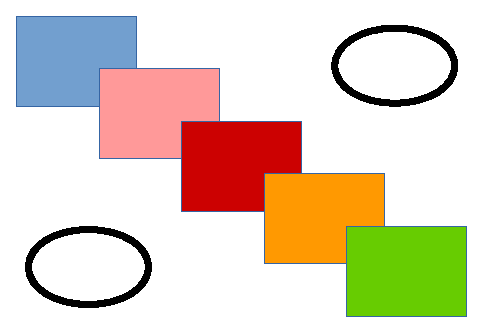
\includegraphics{figures/shapes.eps}
\caption{These are some shapes.}
\label{fig:shapes}
\end{figure}

Good, then we will shall fight in the shade.
Good, then we will shall fight in the shade.
Good, then we will shall fight in the shade.
Good, then we will shall fight in the shade.

% A figure.
\begin{figure}[h]
\centering
\includegraphics[width=\linewidth]{figures/mountains.jpg}
\caption{Majestic mountains.}
\label{fig:mountains}
\end{figure}

% New sub-section.
\subsection{Bullets}

% Start some bullets.
\begin{itemize}

\item All work and no play makes Jack a dull boy.
All work and no play makes Jack a dull boy.

\item All work and no play makes Jack a dull boy.
All work and no play makes Jack a dull boy.

\item All work and no play makes Jack a dull boy.
All work and no play makes Jack a dull boy.

\item All work and no play makes Jack a dull boy.
All work and no play makes Jack a dull boy.

\item All work and no play makes Jack a dull boy.
All work and no play makes Jack a dull boy.

% End the bullets.
\end{itemize}

% New sub-section.
\subsection{Equations}

All work and no play makes Jack a dull boy.

$$
\alpha + \beta = \chi \eqno{(1)}
$$

% New sub-section.
\subsection{Figures}

All work and no play makes Jack a dull boy.
All work and no play makes Jack a dull boy.
All work and no play makes Jack a dull boy.
All work and no play makes Jack a dull boy.
All work and no play makes Jack a dull boy.

\begin{table}[h]
\caption{An Example of a Table}
\label{table_example}
\begin{center}
\begin{tabular}{|c||c|}
\hline
One & Two\\
\hline
Three & Four\\
\hline
\end{tabular}
\end{center}
\end{table}


% New sub-section.
\subsection{Tables}

All work and no play makes Jack a dull boy.
All work and no play makes Jack a dull boy.
All work and no play makes Jack a dull boy.
All work and no play makes Jack a dull boy.
All work and no play makes Jack a dull boy.

\begin{figure}[thpb]
\centering
\framebox{\parbox{3in}{We suggest that you use a text box to insert a graphic (which is ideally a 300 dpi TIFF or EPS file, with all fonts embedded) because, in an document, this method is somewhat more stable than directly inserting a picture.
}}
%\includegraphics[scale=1.0]{figurefile}
\caption{Inductance of oscillation winding on amorphous
magnetic core versus DC bias magnetic field}
\label{figurelabel}
\end{figure}
   
Figure Labels: Use 8 point Times New Roman for Figure labels. Use words rather than symbols or abbreviations when writing Figure axis labels to avoid confusing the reader. As an example, write the quantity Magnetization, or Magnetization, M, not just M. If including units in the label, present them within parentheses. Do not label axes only with units. In the example, write Magnetization (A/m) or Magnetization {A[m(1)]}, not just A/m. Do not label axes with a ratio of quantities and units. For example, write Temperature (K), not Temperature/K.

\section{Conclusion}

All work and no play makes Jack a dull boy.
All work and no play makes Jack a dull boy.
All work and no play makes Jack a dull boy.
All work and no play makes Jack a dull boy.
All work and no play makes Jack a dull boy.
All work and no play makes Jack a dull boy.

\section*{Appendix}

All work and no play makes Jack a dull boy.
All work and no play makes Jack a dull boy.
All work and no play makes Jack a dull boy.
All work and no play makes Jack a dull boy.
All work and no play makes Jack a dull boy.

\section*{Acknowledgment}

All work and no play makes Jack a dull boy.
All work and no play makes Jack a dull boy.
All work and no play makes Jack a dull boy.
All work and no play makes Jack a dull boy.

% Start of the bibliography.
\begin{thebibliography}{99}

\bibitem{c1} G. O. Young, Synthetic structure of industrial plastics (Book style with paper title and editor),   in Plastics, 2nd ed. vol. 3, J. Peters, Ed.  New York: McGraw-Hill, 1964, pp. 15Ð64.

\bibitem{c2} W.-K. Chen, Linear Networks and Systems (Book style).  Belmont, CA: Wadsworth, 1993, pp. 123Ð135.

\bibitem{c3} H. Poor, An Introduction to Signal Detection and Estimation.   New York: Springer-Verlag, 1985, ch. 4.

\bibitem{c4} B. Smith, An approach to graphs of linear forms (Unpublished work style), unpublished.

\bibitem{c5} E. H. Miller, A note on reflector arrays (Periodical styleÑAccepted for publication), IEEE Trans. Antennas Propagat., to be publised.

% End of the bibliography.
\end{thebibliography}

% End of the document.
\end{document}
